%\section{Preliminaries}
%  \label{sec:prelim}

\section{JSON and JSON Schema}
  \label{sec:prelim}

JSON (JavaScript Object Notation) is a lightweight data interchange format commonly used in modern web development and transmission protocols~\citep{bourhis2017json, Pezoa16, peng2011using}. 
A JSON is an unordered set of \textit{key-value} pairs~\citep{peng2011using}. Keys are strings; the values are weakly typed and may be primitive or complex~\citep{baazizi2019parametric}. Figure~\ref{fig:JSONEx} shows a JSON example.

A primitive JSON type is a Boolean ($\mathbb{B}$), a number ($\mathbb{R}$), a string ($\mathbb{S}$), or a \textit{NULL} value~\citep{bourhis2017json}. In Figure~\ref{fig:JSONEx}, the key \textit{type} (line 3) has an  $\mathbb{S}$ (string) value (\textit{`cinematography'}), another example, is the key \textit{year}, which  holds a $\mathbb{R}$ value. 


\begin{figure*}[ht]
    \centering
    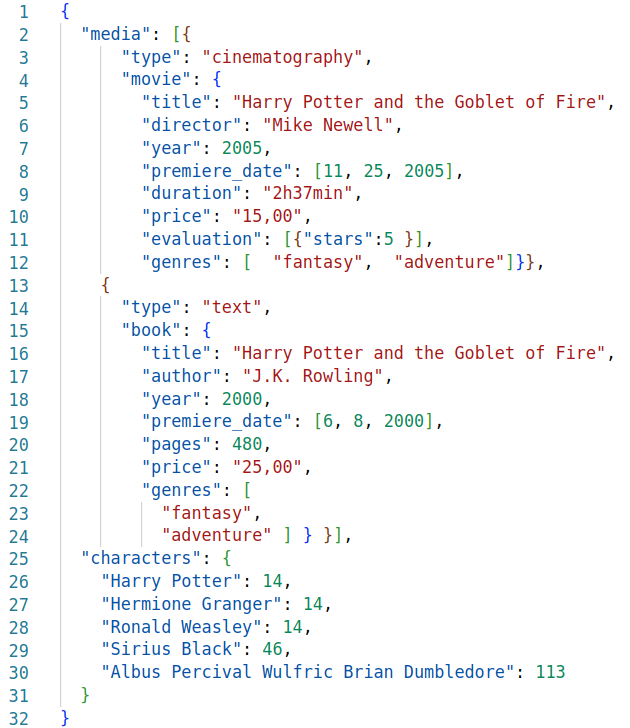
\includegraphics[scale=.45]{Figures/JSONExampleNew.png}
    \caption{An extract of JSON collection: running example}
    \label{fig:JSONEx}
\end{figure*}



A JSON value can also be from a complex type. A complex value type is either an object or an array. A JSON array $\mathcal{A}=[\tau_0, \tau_1,\ldots,\tau_N]$ is a sequence of \textit{N} JSON values (primitive or complex)~\citep{Sp+21}. In Figure~\ref{fig:JSONEx}, the key \textit{media} (line $2$) is an array of complex elements, and the keys \textit{premiere\_date} (lines $8$ and $19$) and \textit{genres} (lines $12$ and $22$) are arrays of primitive elements (\textit{i.e.}, $\mathbb{R}$ and $\mathbb{S}$).

In schema extraction, arrays are extracted as data collections~\citep{Sp+21} since they are a sequence of values. However, in some cases, an array can represent an encoded tuple. 
In the example, the key  \textit{premiere\_date} has three $\mathbb{R}$ values in each occurrence representing a date (month, day, and year) encoded in an array. A naive schema extraction approach will define the field as an ordinary array, losing information about its structure~\citep{Sp+21}.


The last complex type of JSON value is an object. A JSON object $\mathcal{O} = \{ k_1:\tau_1,\ldots,k_N:\tau_N\}$ is a set of keys $k_1...k_N$ mapped to values $\tau_1,\ldots,\tau_N$ of JSON types (primitive or complex)~\citep{Sp+21}. The key \textit{movie} in Figure~\ref{fig:JSONEx} (lines $4$ to $12$) is an example of a complex JSON object. A JSON object is commonly used to encode a tuple since it has a tuple-like structure. 
For example, the key \textit{movie} represents a movie object (or tuple) with attributes \textit{title}, \textit{year}, \textit{director}, and each object of type movie tends to have a very similar structure. However, the key \textit{characters} diverges from this traditional tuple-like structure and encodes a data collection with some characters of the `Harry Potter' universe; if we consider another movie, the list of characters tends to be very different. Considering these two cases, on the one hand, we have a tuple that has a very predictable structure (with a few optional fields), and on the other, we have a more flexible structure that stores a metadata collection.

A JSON Schema is a set of rules that define the schema of a JSON~\citep{Pezoa16}. Hence, a JSON is a set of unordered keys organized hierarchically. The schema defines the keys of a JSON and the kinds (types) of the values from each key~\citep{Sp+21}. The schema generally allows the user to define whether an attribute is optional or mandatory. Also, the schema allows the definition of occurrences of enumerations and tagged unions. 

We consider an enumeration of a field with multiple occurrences and a low variability of values. For example, in Figure~\ref{fig:JSONEx}, the key \textit{type} (lines $3$ and $14$) stores the  \textit{media} type, assuming just two possible values: `cinematography' or `text'. Any other value can not be accepted for the field  \textit{type}.

A tagged union is a particular type of enumeration that allows conditional occurrences of one or more fields based on the value of a previous key/element ~\citep{Sp+21}. For example, in Figure~\ref{fig:JSONEx}, the key \textit{type} is followed by either the key \textit{movie} (line $4$) or \textit{book} (line $15$), depending on whether the \textit{type} is `cinematography' or `text'.

Our approach intends to consider all the facets presented here to discover a schema from a JSON collection, as shown in following sections.